\documentclass{article}
\usepackage{listings}
\usepackage{xcolor}
\usepackage{graphicx} % Required for inserting images
\usepackage{tikz} % Drawing
\usepackage[backend=biber,style=apa]{biblatex}
\usepackage{amsmath}

\lstset{ 
  language=R,
  backgroundcolor=\color{white},   
  basicstyle=\footnotesize\ttfamily,    
  breaklines=true,                    
  captionpos=b,                     
  keepspaces=true,                   
  numbers=left,                     
  numberstyle=\tiny\color{gray},  
  stringstyle=\color{purple},     
  commentstyle=\color{gray},  
  keywordstyle=\color{blue},  
  showstringspaces=false
}

% load bib
\addbibresource{reference.bib}

\title{BKT: A Bayesian Knowledge Tracing Package for the R Environment}
\author{Yuhao Yuan, Biying Zhou, Feng Ji}
\date{\today}

\begin{document}

\maketitle

% some notes
\begin{itemize}
    \item Target Journal: Journal of Statistical Software, Behavior Research Methods, Or Applied Psychological Measurement
    \item \textbf{Storyline} Introduce BKT and its variant, showcase its usefulness in an empirical data and/or a simulated data $\rightarrow$ give a simple tutorial involving how to use it in R.
\end{itemize}
\section{Introduction}

The advent of digital technologies has led to an unprecedented increase in the availability and granularity of educational assessment data. These data, collected from diverse learning environments such as online courses, intelligent tutoring systems, and classroom-based assessments, provide detailed insights into students' learning processes. With the growing emphasis on evidence-based approaches in education, this wealth of data has opened new avenues for research and practice, allowing educators and researchers to address fundamental questions about learning and knowledge acquisition.

One critical application of educational assessment data lies in understanding how students learn over time and predicting their future performance. Traditional methods of assessment often provide only static snapshots of a learner's knowledge at specific points in time. However, as the demand for personalized and adaptive learning systems increases, there is a pressing need for dynamic models that can capture the evolving nature of student knowledge. This is where Bayesian Knowledge Tracing (BKT) and its variants play a pivotal role.

BKT offers a probabilistic framework for modeling the progression of a learner's knowledge state (\cite{corbett1994knowledge}). By leveraging sequential data on student performance, BKT enables the estimation of underlying knowledge states and provides predictions about future responses. These capabilities make it an essential tool for adaptive learning systems, as they can identify individual learning needs and recommend tailored interventions. Moreover, BKT's simplicity and interpretability have contributed to its widespread adoption in both research and practice.

Despite its widespread utility, BKT is not without limitations. Researchers have proposed various extensions and modifications to address issues such as model flexibility, parameter estimation, and the integration of additional features like forgetting or partial knowledge. These advancements have further broadened the applicability of BKT to more complex and realistic educational scenarios.

To facilitate the use of BKT in educational research and practical applications, we have developed the BKT R package. This package provides an easy-to-use implementation of Bayesian Knowledge Tracing, allowing researchers and educators to easily apply BKT models to their own data. With functionalities for parameter estimation, model fitting, and evaluation, the BKT R package streamlines the process of using BKT in diverse educational settings. It is designed to integrate seamlessly with the R environment, offering flexibility for further customization and enhancement.

This paper aims to provide a comprehensive overview of BKT and its variants, showcasing their usefulness through empirical and simulated data analyses. Additionally, we offer a practical tutorial on implementing BKT using the BKT R package, enabling researchers and practitioners to leverage this powerful model in their own work. By bridging theoretical insights with practical applications, this paper seeks to contribute to the growing body of knowledge on dynamic learning models and their role in advancing educational research and practice.


\section{Model description}

\subsection{Bayesian Knowledge Tracing}
BKT (Bayesian Knowledge Tracing) is a probabilistic model designed to track a learner’s state of knowledge over time, specifically focusing on transitions between 'unknown' and 'known' states for a particular skill or concept. BKT assumes that a learner has a probability of transitioning from an unknown state to a known state based on the correctness of their responses during learning activities. Here, we provide detailed explanations of the learning process as abstracted by the BKT model.

In general, people acquire knowledge by engaging in learning activities. Learner's knowledge state can be observed by changes in their performance on these activities. This learning process is illustrated in Figure 1.

\begin{center}
    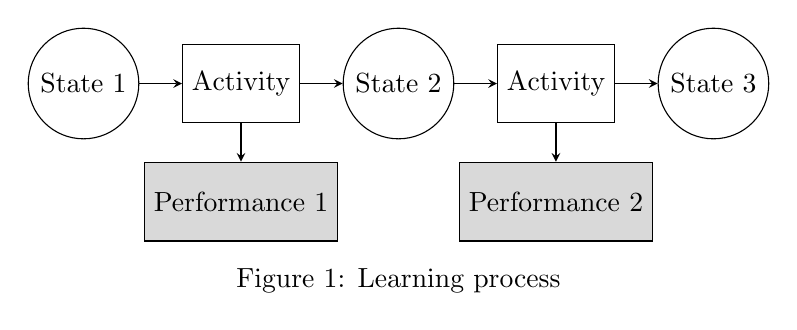
\begin{tikzpicture}
        % Define styles
        \tikzset{
            state/.style={circle, draw, minimum size=1cm},
            activity/.style={rectangle, draw, minimum size=1cm},
            performance/.style={rectangle, draw, fill=gray!30, minimum size=1cm},
            arrow/.style={->,>=stealth}
        }
        
        % Nodes
        \node[state] (state_node_1) at (0,0) {State 1};
        \node[activity] (activity_node_1) at (2,0) {Activity};
        \node[performance] (performance_node_1) at (2,-1.5) {Performance 1};
        \node[state] (state_node_2) at (4,0) {State 2};
        
        \node[activity] (activity_node_2) at (6,0) {Activity};
        \node[performance] (performance_node_2) at (6,-1.5) {Performance 2};
        \node[state] (state_node_3) at (8,0) {State 3};
        
        % Arrows
        \draw[arrow] (state_node_1) -- (activity_node_1);
        \draw[arrow] (activity_node_1) -- (state_node_2);
        \draw[arrow] (activity_node_1) -- (performance_node_1);
        \draw[arrow] (state_node_2) -- (activity_node_2);
        \draw[arrow] (activity_node_2) -- (state_node_3);
        \draw[arrow] (activity_node_2) -- (performance_node_2);
    
        % Footnote
        \node at (4,-2.5) {Figure 1: Learning process};
    \end{tikzpicture}
\end{center}

Another assumption of the BKT model is the binary nature of learning states and the impact of activities on these states. BKT assumes that a learner is either in a known state or an unknown state. By participating in an activity, a learner in the unknown state has a chance to transition to the known state. Therefore, learning activities cause three types of state changes: remaining known, learning (transitioning from unknown to known), and remaining unknown. This is illustrated in Figure 2. Note that the transition from the unknown state to the known state represents the learning process as a hidden Markov model in the BKT framework.

\begin{center}
    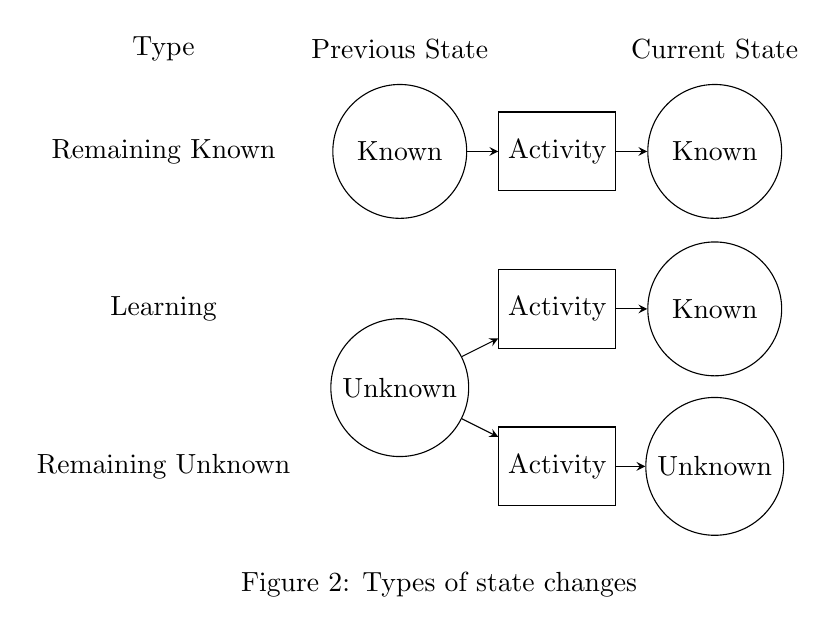
\begin{tikzpicture}
        % Define styles
        \tikzset{
            state/.style={circle, draw, minimum size=1.7cm},
            activity/.style={rectangle, draw, minimum size=1cm},
            arrow/.style={->,>=stealth}
        }
        
        % Nodes
        \node[] () at (-3,1.3) {Type};
        \node[] () at (0,1.3) {Previous State};
        \node[] () at (4,1.3) {Current State};

        \node[] () at (-3,0) {Remaining Known};
        \node[state] (state_node_1) at (0,0) {Known};
        \node[activity] (activity_node_1) at (2,0) {Activity};
        \node[state] (state_node_2) at (4,0) {Known};
        
        \node[] () at (-3,-2) {Learning};
        \node[state] (state_node_3) at (0,-3) {Unknown};
        \node[activity] (activity_node_2) at (2,-2) {Activity};
        \node[state] (state_node_4) at (4,-2) {Known};
        
        \node[] () at (-3,-4) {Remaining Unknown};
        % \node[state] (state_node_5) at (0,-4) {Unknown};
        \node[activity] (activity_node_3) at (2,-4) {Activity};
        \node[state] (state_node_6) at (4,-4) {Unknown};
        
        % Arrows
        \draw[arrow] (state_node_1) -- (activity_node_1);
        \draw[arrow] (activity_node_1) -- (state_node_2);
        \draw[arrow] (state_node_3) -- (activity_node_2);
        \draw[arrow] (activity_node_2) -- (state_node_4);
        \draw[arrow] (state_node_3) -- (activity_node_3);
        \draw[arrow] (activity_node_3) -- (state_node_6);
    
        % Footnote
        \node at (0.5,-5.5) {Figure 2: Types of state changes};
    \end{tikzpicture}
\end{center}

One can infer a learner’s knowledge state by observing their performance on activities. However, there are two common scenarios to consider: a learner in an unknown state answering correctly (guessing) and a learner in a known state answering incorrectly (slipping). The relationship between activity performance and knowledge state is shown in Figure 3.

\begin{center}
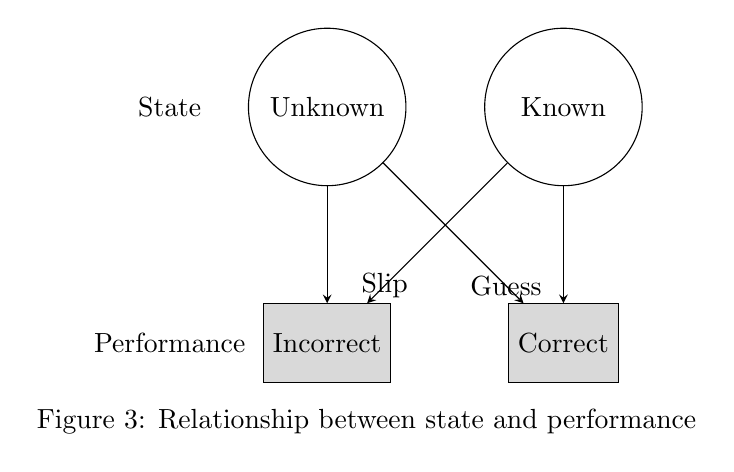
\begin{tikzpicture}
    % Define styles
    \tikzset{
        state/.style={circle, draw, minimum size=2cm},
        performance/.style={rectangle, draw, fill=gray!30, minimum size=1cm},
        arrow/.style={->,>=stealth}
    }
    
    % Nodes
    \node[] (state_label) at (-1,0) {State};
    \node[] (performance_label) at (-1,-3) {Performance};
    \node[state] (not_known) at (1,0) {Unknown};
    \node[state] (known) at (4,0) {Known};
    \node[performance] (incorrect) at (1,-3) {Incorrect};
    \node[performance] (correct) at (4,-3) {Correct};
    
    % Arrows
    \draw[arrow] (not_known) -- (incorrect);
    \draw[arrow] (not_known) -- (correct) node[very near end] {Guess};
    \draw[arrow] (known) -- (correct);
    \draw[arrow] (known) -- (incorrect) node[very near end] {Slip};

    % Footnote
    \node at (1.5,-4) {Figure 3: Relationship between state and performance};
\end{tikzpicture}
\end{center}

BKT provides a static approach, using specific and quantified probability descriptions to calculate the likelihood of the learning process.

In BKT terminology, we define the following:

1. \textbf{Answer}  
The answer for an activity, denoted as \( a \), represents the response given by a learner during the activity. According to BKT assumptions, its value is binary, either 0 or 1.

The variable \textbf{Answer} is the only input variable in this model.

2. \textbf{Prior}  
The prior rate, \( P_p \), represents the probability that a learner is initially in the known state.

3. \textbf{Learn}  
The learning rate, \( P_l \), indicates the probability that a learner transitions to the known state through learning.

4. \textbf{Slip}  
The slip rate, \( P_s \), denotes the probability that a learner in the known state answers incorrectly.

5. \textbf{Guess}  
The guess rate, \( P_g \), represents the probability that a learner in the unknown state answers correctly.

These four variables (\textbf{Prior} \textbf{Learn} \textbf{Slip} \textbf{Guess}) are global parameters that remain constant throughout the model.

6. \textbf{Know}  
The known rate, \( \theta \), reflects the probability that a learner is in the known state. Unlike the other parameters, \textbf{Know} is dynamic and updates iteratively as the model progresses.

For a learning process with an answer vector \( (a_1, a_2, \dots, a_s) \), the likelihood of the sequence in the BKT model is calculated as follows:

For each answer \( a_i \), let \(\theta_{i}\) denote the known rate before the \(i\)-th activity, and \(\theta_{i+1}\) the known rate after the \(i\)-th activity. Note \(\theta_1 = P_p\). The iteration of \(\theta_{i+1}\) is as follows:

First, calculate \(\theta'\), the updated known rate using Bayes' rule based on the observed answer \( a_i \):
\[
\theta' = 
\begin{cases} 
    \frac{\theta_{i} P_s}{\theta_{i} P_s + (1 - \theta_{i}) (1 - P_g)}, & \text{if } a_i = 0 \\[10pt]
    \frac{\theta_{i} (1 - P_s)}{\theta_{i} (1 - P_s) + (1 - \theta_{i}) P_g}, & \text{if } a_i = 1 
\end{cases}
\]

Figure 4 illustrates the Bayes update process.

\begin{center}
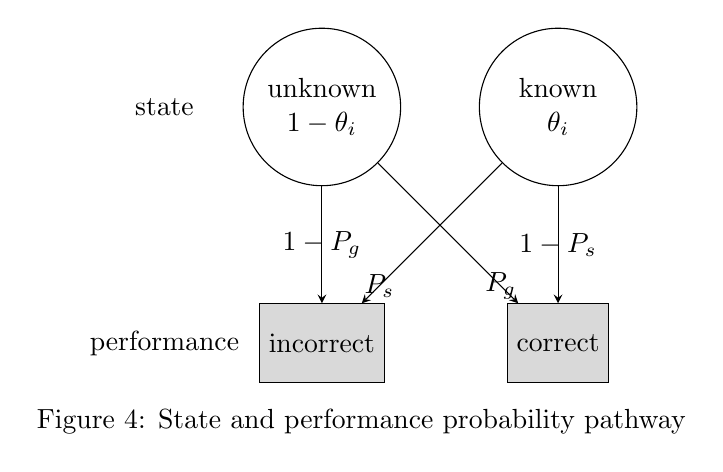
\begin{tikzpicture}
    % Define styles
    \tikzset{
        state/.style={circle, draw, minimum size=2cm},
        performance/.style={rectangle, draw, fill=gray!30, minimum size=1cm},
        arrow/.style={->,>=stealth}
    }
    
    % Nodes
    \node[] (state_node) at (-1,0) {state};
    \node[] (performance_node) at (-1,-3) {performance};
    \node[state] (not_known) at (1,0) {\parbox{1.5cm}{\centering unknown \\ \(1 - \theta_i\)}};
    \node[state] (known) at (4,0) {\parbox{1.5cm}{\centering known \\ \(\theta_{i}\)}};
    \node[performance] (incorrect) at (1,-3) {incorrect};
    \node[performance] (correct) at (4,-3) {correct};
    
    % Arrows
    \draw[arrow] (not_known) -- (incorrect) node[midway] {$1 - P_g$};
    \draw[arrow] (not_known) -- (correct) node[very near end] {$P_g$};
    \draw[arrow] (known) -- (correct) node[midway] {$1 - P_s$};
    \draw[arrow] (known) -- (incorrect) node[very near end] {$P_s$};

    % Figure label
    \node at (1.5,-4) {Figure 4: State and performance probability pathway};
\end{tikzpicture}
\end{center}

Then, update \(\theta_{i+1}\) by incorporating the potential learning effect based on \(\theta'\).

\[
\theta_{i+1} = \theta' + (1 - \theta') P_l    
\]

Now we know all learn rate before each activity \(\theta_i\), we use them to calculate the probability of each activity outcome.

\[
    Lik_i = 
    \begin{cases} 
        P_s \theta_{i} + (1 - P_g) (1 - \theta_i), & \text{if } a_i = 0 \\[10pt]
        (1 - P_s) \theta_{i} + P_g (1 - \theta_i), & \text{if } a_i = 1 
    \end{cases}
\]

So the total learn process's probability is

\[
    Lik = \prod Lik_i
\]

We can utilize the standard expectation-maximization (EM) algorithm to determine the global parameters (\(P_p, P_l, P_s, P_g\)). The EM algorithm is particularly well-suited for this task because the knowledge state of the learner is a latent variable—an unobservable factor that influences the observed performance. Directly maximizing $Lik$ is challenging due to the need to sum over all possible latent states. The EM algorithm simplifies this by iteratively estimating the expected contribution of latent states (E-step) and optimizing the parameters given these estimates (M-step), ensuring a systematic and efficient approach to converge to the optimal parameter estimates. The detailed computational steps of the EM algorithm are provided in Section Estimation.

The basic Bayesian Knowledge Tracing (BKT) model is involved here. However, it should be noted that the basic BKT model has certain limitations. The most significant issue is that it presupposes a large number of global parameters. As a result of applying these global parameters to local scenarios, numerous variants of the BKT model have emerged. At the same time, by expanding the functionality of the BKT model, some variant BKT models have also been proposed.

\subsection{BKT Variants}

% variant              name                                                        url              
% forget               Knowledge Tracing and Forgets Models                https://dl.acm.org/doi/abs/10.1145/3511808.3557622
% multilearn         Item Learning Effect Model                            http://ml4ed.cc/attachments/XuY.pdf
% multiguess        Item Difficulty Effect Mode                            https://link.springer.com/chapter/10.1007/978-3-642-22362-4_21
% multiprior          Prior per Student Model                              https://link.springer.com/chapter/10.1007/978-3-642-13470-8_24
% multipair           Item Order Effect Model                              https://eric.ed.gov/?id=ED539081
% fixed
Before introducing variants, we need to know how the basic BKT handles learning processes of multiple students.

In general, BKT calculate each student learning process likelihood individually while using same global parameters as shown in Figure 5.

\begin{center}
    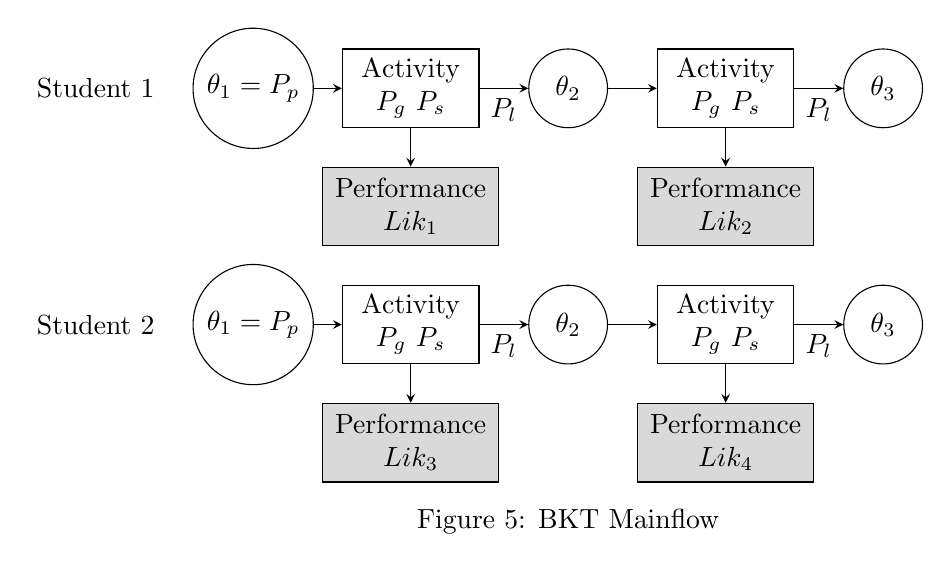
\begin{tikzpicture}
        % Define styles
        \tikzset{
            state/.style={circle, draw, minimum size=1cm},
            activity/.style={rectangle, draw, minimum size=1cm},
            performance/.style={rectangle, draw, fill=gray!30, minimum size=1cm},
            arrow/.style={->,>=stealth}
        }
        
        % Nodes
        \node[] () at (-2,0) {Student 1};
        \node[state] (state_node_1) at (0,0) {$\theta_1 = P_p$};
        \node[activity] (activity_node_1) at (2,0) {\parbox{1.5cm}{\centering Activity \\ $P_g \ P_s$}};
        \node[performance] (performance_node_1) at (2,-1.5) {\parbox{2cm}{\centering Performance \\ $Lik_1$}};
        \node[state] (state_node_2) at (4,0) {$\theta_2$};
        
        \node[activity] (activity_node_2) at (6,0) {\parbox{1.5cm}{\centering Activity \\ $P_g \ P_s$}};
        \node[performance] (performance_node_2) at (6,-1.5) {\parbox{2cm}{\centering Performance \\ $Lik_2$}};
        \node[state] (state_node_3) at (8,0) {$\theta_3$};
        
        % Arrows
        \draw[arrow] (state_node_1) -- (activity_node_1);
        \draw[arrow] (activity_node_1) -- (state_node_2) node[midway, below] {$P_l$};
        \draw[arrow] (activity_node_1) -- (performance_node_1);
        \draw[arrow] (state_node_2) -- (activity_node_2);
        \draw[arrow] (activity_node_2) -- (state_node_3) node[midway, below] {$P_l$};
        \draw[arrow] (activity_node_2) -- (performance_node_2);
    

        % student 2
        \node[] () at (-2,-3) {Student 2};
        \node[state] (state_node_2) at (0,-3) {$\theta_1 = P_p$};
        \node[activity] (activity_node_2) at (2,-3) {\parbox{1.5cm}{\centering Activity \\ $P_g \ P_s$}};
        \node[performance] (performance_node_2) at (2,-4.5) {\parbox{2cm}{\centering Performance \\ $Lik_3$}};
        \node[state] (state_node_3) at (4,-3) {$\theta_2$};
        \node[activity] (activity_node_3) at (6,-3) {\parbox{1.5cm}{\centering Activity \\ $P_g \ P_s$}};
        \node[performance] (performance_node_3) at (6,-4.5) {\parbox{2cm}{\centering Performance \\ $Lik_4$}};
        \node[state] (state_node_4) at (8,-3) {$\theta_3$};
        \draw[arrow] (state_node_2) -- (activity_node_2);
        \draw[arrow] (activity_node_2) -- (state_node_3) node[midway, below] {$P_l$};
        \draw[arrow] (activity_node_2) -- (performance_node_2);
        \draw[arrow] (state_node_3) -- (activity_node_3);
        \draw[arrow] (activity_node_3) -- (state_node_4) node[midway, below] {$P_l$};
        \draw[arrow] (activity_node_3) -- (performance_node_3);

        % Footnote
        \node at (4,-5.5) {Figure 5: BKT Mainflow};
    \end{tikzpicture}
\end{center}

\subsubsection{Multiple Prior}
The Prior Per Student (PPS) Model (\cite{multiprior}) is based on BKT that focuses on individualizing the prior. The BKT assumes all student share same prior rate, the global parameter \( P_p \). The PPS localizes prior rate into each student.

The main difference in the model description lies in the initial known rate.

For each student \( j \), let \( P_{p_j} \) denote their individual prior rate. Let \(\theta_{i_j}\) denote the known rate before the \(i\)-th activity of student \(j\).
Note \(\theta_{1_j} = P_{p_j} \).

The mainflow of PPS is illustrated in Figure 6. Note different student uses different initial known rate \(\theta_1\).

\begin{center}
    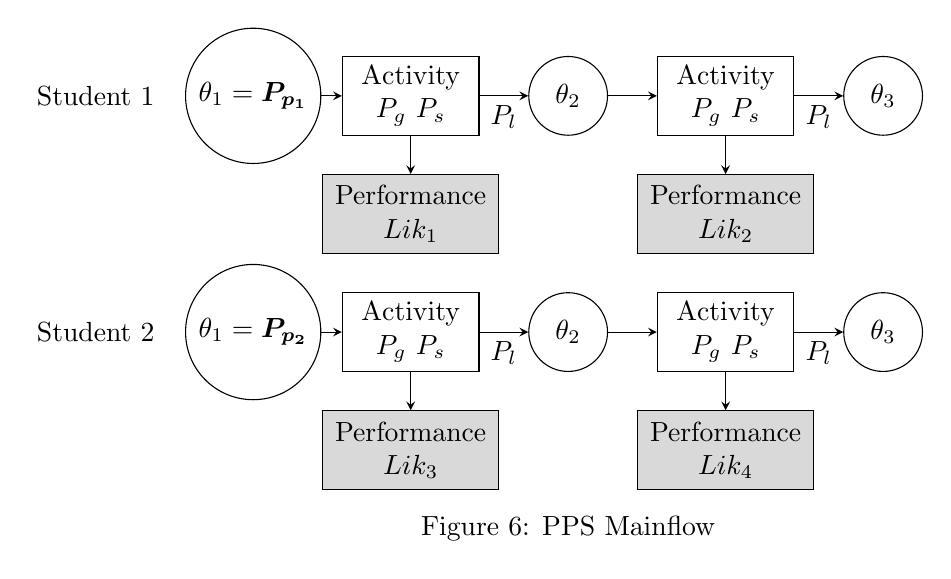
\begin{tikzpicture}
        % Define styles
        \tikzset{
            state/.style={circle, draw, minimum size=1cm},
            activity/.style={rectangle, draw, minimum size=1cm},
            performance/.style={rectangle, draw, fill=gray!30, minimum size=1cm},
            arrow/.style={->,>=stealth}
        }
        
        % Nodes
        \node[] () at (-2,0) {Student 1};
        \node[state] (state_node_1) at (0,0) {$\theta_1 = \boldsymbol{P_{p_1}}$};
        \node[activity] (activity_node_1) at (2,0) {\parbox{1.5cm}{\centering Activity \\ $P_g \ P_s$}};
        \node[performance] (performance_node_1) at (2,-1.5) {\parbox{2cm}{\centering Performance \\ $Lik_1$}};
        \node[state] (state_node_2) at (4,0) {$\theta_2$};
        
        \node[activity] (activity_node_2) at (6,0) {\parbox{1.5cm}{\centering Activity \\ $P_g \ P_s$}};
        \node[performance] (performance_node_2) at (6,-1.5) {\parbox{2cm}{\centering Performance \\ $Lik_2$}};
        \node[state] (state_node_3) at (8,0) {$\theta_3$};
        
        % Arrows
        \draw[arrow] (state_node_1) -- (activity_node_1);
        \draw[arrow] (activity_node_1) -- (state_node_2) node[midway, below] {$P_l$};
        \draw[arrow] (activity_node_1) -- (performance_node_1);
        \draw[arrow] (state_node_2) -- (activity_node_2);
        \draw[arrow] (activity_node_2) -- (state_node_3) node[midway, below] {$P_l$};
        \draw[arrow] (activity_node_2) -- (performance_node_2);
    

        % student 2
        \node[] () at (-2,-3) {Student 2};
        \node[state] (state_node_2) at (0,-3) {$\theta_1 = \boldsymbol{P_{p_2}}$};
        \node[activity] (activity_node_2) at (2,-3) {\parbox{1.5cm}{\centering Activity \\ $P_g \ P_s$}};
        \node[performance] (performance_node_2) at (2,-4.5) {\parbox{2cm}{\centering Performance \\ $Lik_3$}};
        \node[state] (state_node_3) at (4,-3) {$\theta_2$};
        \node[activity] (activity_node_3) at (6,-3) {\parbox{1.5cm}{\centering Activity \\ $P_g \ P_s$}};
        \node[performance] (performance_node_3) at (6,-4.5) {\parbox{2cm}{\centering Performance \\ $Lik_4$}};
        \node[state] (state_node_4) at (8,-3) {$\theta_3$};
        \draw[arrow] (state_node_2) -- (activity_node_2);
        \draw[arrow] (activity_node_2) -- (state_node_3) node[midway, below] {$P_l$};
        \draw[arrow] (activity_node_2) -- (performance_node_2);
        \draw[arrow] (state_node_3) -- (activity_node_3);
        \draw[arrow] (activity_node_3) -- (state_node_4) node[midway, below] {$P_l$};
        \draw[arrow] (activity_node_3) -- (performance_node_3);

        % Footnote
        \node at (4,-5.5) {Figure 6: PPS Mainflow};
    \end{tikzpicture}
\end{center}

\subsubsection{Multiple Learn}

The Item Learning Effect (ILE) Model (\cite{multilearn}) is based on BKT that focuses on individualizing the learning rate. The BKT assumes all item (activity) share same learning rate, the global parameter \( P_l \). The ILE localizes learning rate into each item.

The main difference in the model description lies in the learning rate.

For each activity \( j \), let \( P_{l_j} \) denotes the learning rate.

The mainflow of ILE is illustrated in Figure 7. Note there are three different activities, 1, 2 and 3.

\begin{center}
    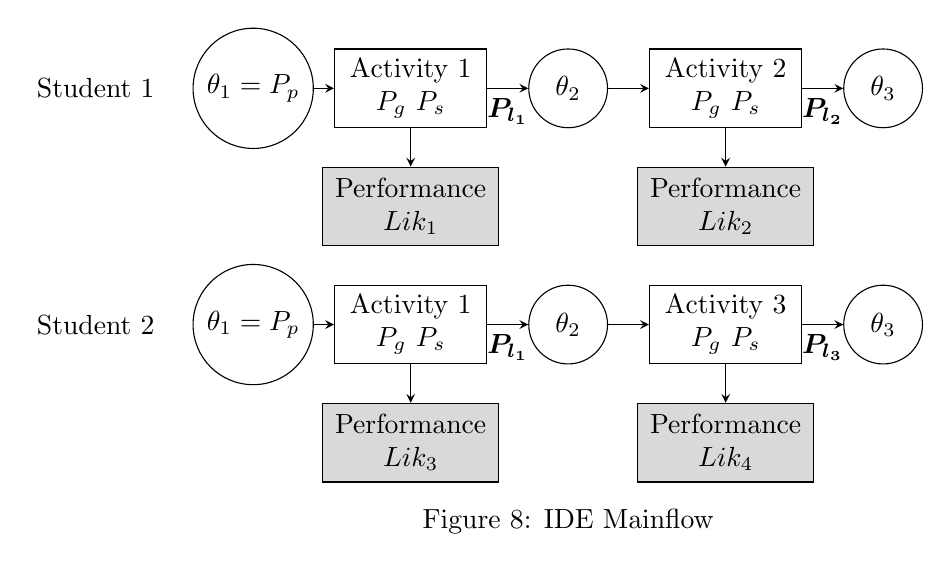
\begin{tikzpicture}
        % Define styles
        \tikzset{
            state/.style={circle, draw, minimum size=1cm},
            activity/.style={rectangle, draw, minimum size=1cm},
            performance/.style={rectangle, draw, fill=gray!30, minimum size=1cm},
            arrow/.style={->,>=stealth}
        }
        
        % Nodes
        \node[] () at (-2,0) {Student 1};
        \node[state] (state_node_1) at (0,0) {$\theta_1 = P_p$};
        \node[activity] (activity_node_1) at (2,0) {\parbox{1.7cm}{\centering Activity 1 \\ ${P_{g} \ P_{s}}$}};
        \node[performance] (performance_node_1) at (2,-1.5) {\parbox{2cm}{\centering Performance \\ $Lik_1$}};
        \node[state] (state_node_2) at (4,0) {$\theta_2$};
        
        \node[activity] (activity_node_2) at (6,0) {\parbox{1.7cm}{\centering Activity 2 \\ ${P_{g} \ P_{s}}$}};
        \node[performance] (performance_node_2) at (6,-1.5) {\parbox{2cm}{\centering Performance \\ $Lik_2$}};
        \node[state] (state_node_3) at (8,0) {$\theta_3$};
        
        % Arrows
        \draw[arrow] (state_node_1) -- (activity_node_1);
        \draw[arrow] (activity_node_1) -- (state_node_2) node[midway, below] {$\boldsymbol{P_{l_1}}$};
        \draw[arrow] (activity_node_1) -- (performance_node_1);
        \draw[arrow] (state_node_2) -- (activity_node_2);
        \draw[arrow] (activity_node_2) -- (state_node_3) node[midway, below] {$\boldsymbol{P_{l_2}}$};
        \draw[arrow] (activity_node_2) -- (performance_node_2);
    

        % student 2
        \node[] () at (-2,-3) {Student 2};
        \node[state] (state_node_2) at (0,-3) {$\theta_1 = P_p$};
        \node[activity] (activity_node_2) at (2,-3) {\parbox{1.7cm}{\centering Activity 1 \\ ${P_{g} \ P_{s}}$}};
        \node[performance] (performance_node_2) at (2,-4.5) {\parbox{2cm}{\centering Performance \\ $Lik_3$}};
        \node[state] (state_node_3) at (4,-3) {$\theta_2$};
        \node[activity] (activity_node_3) at (6,-3) {\parbox{1.7cm}{\centering Activity 3 \\ ${P_{g} \ P_{s}}$}};
        \node[performance] (performance_node_3) at (6,-4.5) {\parbox{2cm}{\centering Performance \\ $Lik_4$}};
        \node[state] (state_node_4) at (8,-3) {$\theta_3$};
        \draw[arrow] (state_node_2) -- (activity_node_2);
        \draw[arrow] (activity_node_2) -- (state_node_3) node[midway, below] {$\boldsymbol{P_{l_1}}$};
        \draw[arrow] (activity_node_2) -- (performance_node_2);
        \draw[arrow] (state_node_3) -- (activity_node_3);
        \draw[arrow] (activity_node_3) -- (state_node_4) node[midway, below] {$\boldsymbol{P_{l_3}}$};
        \draw[arrow] (activity_node_3) -- (performance_node_3);

        % Footnote
        \node at (4,-5.5) {Figure 8: IDE Mainflow};
    \end{tikzpicture}
\end{center}


\subsubsection{Multiple Pair}

The Item Order Effect (IOE) Model (\cite{multipair}) is based on BKT that focuses on individualizing the learning rate. The BKT assumes all item (activity) share same learning rate, the global parameter \( P_l \). The IOE localizes learning rate into each item pairs.

The main difference in the model description lies in the learning rate.

For each activity \( i \) and activity \( j \), let \( P_{l_{ij}} \) denotes the learning rate from activity \( i \) to activity \( j \). Note \( P_{l_{0j}} \) refers initial activity learn rate.

The mainflow of ILE is illustrated in Figure 9. Note there are three different activities, 1, 2 and 3 with most 6 pairs.

\begin{center}
    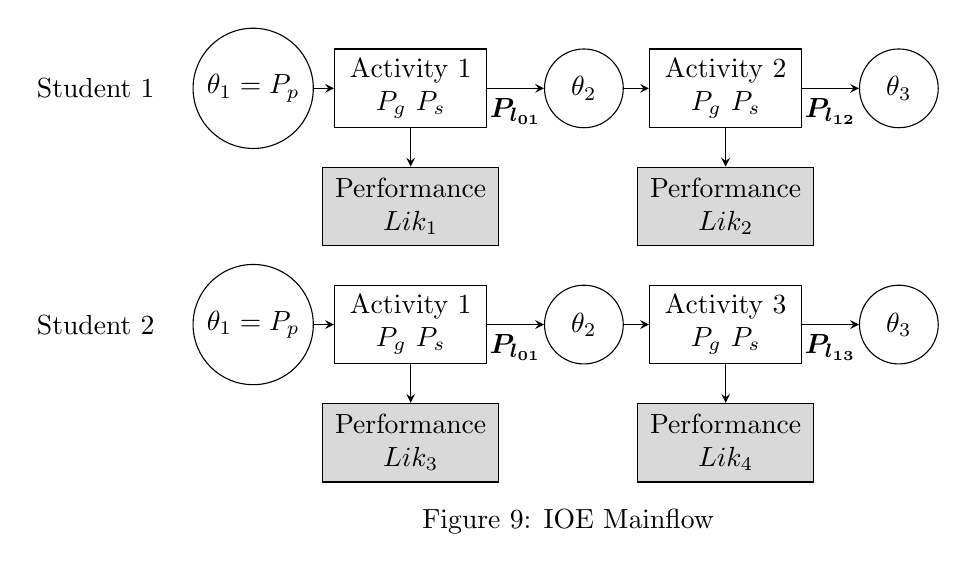
\begin{tikzpicture}
        % Define styles
        \tikzset{
            state/.style={circle, draw, minimum size=1cm},
            activity/.style={rectangle, draw, minimum size=1cm},
            performance/.style={rectangle, draw, fill=gray!30, minimum size=1cm},
            arrow/.style={->,>=stealth}
        }
        
        % Nodes
        \node[] () at (-2,0) {Student 1};
        \node[state] (state_node_1) at (0,0) {$\theta_1 = P_p$};
        \node[activity] (activity_node_1) at (2,0) {\parbox{1.7cm}{\centering Activity 1 \\ ${P_{g} \ P_{s}}$}};
        \node[performance] (performance_node_1) at (2,-1.5) {\parbox{2cm}{\centering Performance \\ $Lik_1$}};
        \node[state] (state_node_2) at (4.2,0) {$\theta_2$};
        
        \node[activity] (activity_node_2) at (6,0) {\parbox{1.7cm}{\centering Activity 2 \\ ${P_{g} \ P_{s}}$}};
        \node[performance] (performance_node_2) at (6,-1.5) {\parbox{2cm}{\centering Performance \\ $Lik_2$}};
        \node[state] (state_node_3) at (8.2,0) {$\theta_3$};
        
        % Arrows
        \draw[arrow] (state_node_1) -- (activity_node_1);
        \draw[arrow] (activity_node_1) -- (state_node_2) node[midway, below] {$\boldsymbol{P_{l_{01}}}$};
        \draw[arrow] (activity_node_1) -- (performance_node_1);
        \draw[arrow] (state_node_2) -- (activity_node_2);
        \draw[arrow] (activity_node_2) -- (state_node_3) node[midway, below] {$\boldsymbol{P_{l_{12}}}$};
        \draw[arrow] (activity_node_2) -- (performance_node_2);
    

        % student 2
        \node[] () at (-2,-3) {Student 2};
        \node[state] (state_node_2) at (0,-3) {$\theta_1 = P_p$};
        \node[activity] (activity_node_2) at (2,-3) {\parbox{1.7cm}{\centering Activity 1 \\ ${P_{g} \ P_{s}}$}};
        \node[performance] (performance_node_2) at (2,-4.5) {\parbox{2cm}{\centering Performance \\ $Lik_3$}};
        \node[state] (state_node_3) at (4.2,-3) {$\theta_2$};
        \node[activity] (activity_node_3) at (6,-3) {\parbox{1.7cm}{\centering Activity 3 \\ ${P_{g} \ P_{s}}$}};
        \node[performance] (performance_node_3) at (6,-4.5) {\parbox{2cm}{\centering Performance \\ $Lik_4$}};
        \node[state] (state_node_4) at (8.2,-3) {$\theta_3$};
        \draw[arrow] (state_node_2) -- (activity_node_2);
        \draw[arrow] (activity_node_2) -- (state_node_3) node[midway, below] {$\boldsymbol{P_{l_{01}}}$};
        \draw[arrow] (activity_node_2) -- (performance_node_2);
        \draw[arrow] (state_node_3) -- (activity_node_3);
        \draw[arrow] (activity_node_3) -- (state_node_4) node[midway, below] {$\boldsymbol{P_{l_{13}}}$};
        \draw[arrow] (activity_node_3) -- (performance_node_3);

        % Footnote
        \node at (4,-5.5) {Figure 9: IOE Mainflow};
    \end{tikzpicture}
\end{center}


\subsubsection{Multiple Guess and Slip}

The Item Difficulty Effect (IDE) Model (\cite{multiguess}) is based on BKT that focuses on individualizing the guess and slip. The BKT assumes all item (activity) share same guess and slip rate, the global parameter \( P_g \) and \( P_s \). The IDE localizes guess and slip rate into each item.

The main difference in the model description lies in the guess and slip rate.

For each activity \( j \), let \( P_{g_j} \) denotes the guess rate and \( P_{s_j} \) denotes the slip rate.

The mainflow of PPS is illustrated in Figure 10. Note there are three different activities, 1, 2 and 3.

\begin{center}
    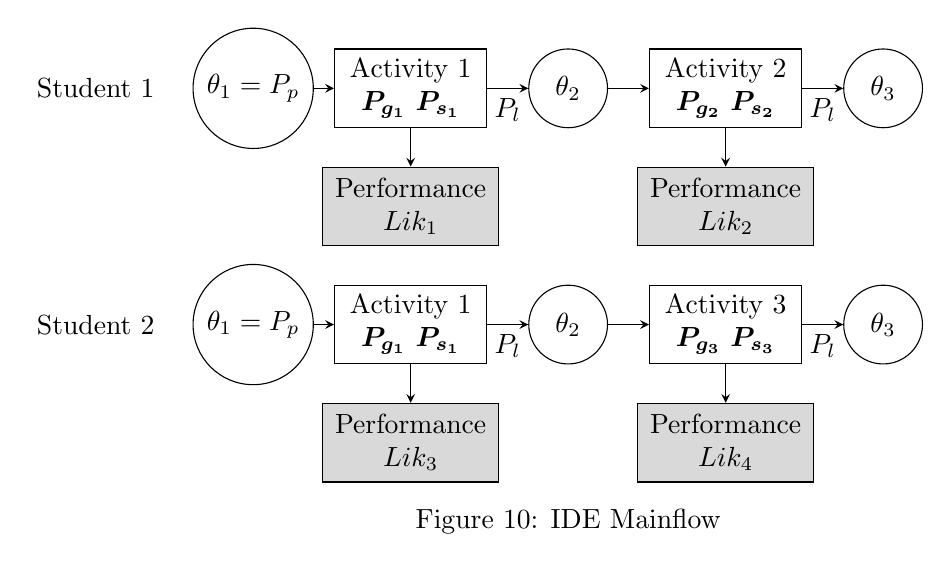
\begin{tikzpicture}
        % Define styles
        \tikzset{
            state/.style={circle, draw, minimum size=1cm},
            activity/.style={rectangle, draw, minimum size=1cm},
            performance/.style={rectangle, draw, fill=gray!30, minimum size=1cm},
            arrow/.style={->,>=stealth}
        }
        
        % Nodes
        \node[] () at (-2,0) {Student 1};
        \node[state] (state_node_1) at (0,0) {$\theta_1 = P_p$};
        \node[activity] (activity_node_1) at (2,0) {\parbox{1.7cm}{\centering Activity 1 \\ $\boldsymbol{P_{g_1} \ P_{s_1}}$}};
        \node[performance] (performance_node_1) at (2,-1.5) {\parbox{2cm}{\centering Performance \\ $Lik_1$}};
        \node[state] (state_node_2) at (4,0) {$\theta_2$};
        
        \node[activity] (activity_node_2) at (6,0) {\parbox{1.7cm}{\centering Activity 2 \\ $\boldsymbol{P_{g_2} \ P_{s_2}}$}};
        \node[performance] (performance_node_2) at (6,-1.5) {\parbox{2cm}{\centering Performance \\ $Lik_2$}};
        \node[state] (state_node_3) at (8,0) {$\theta_3$};
        
        % Arrows
        \draw[arrow] (state_node_1) -- (activity_node_1);
        \draw[arrow] (activity_node_1) -- (state_node_2) node[midway, below] {$P_l$};
        \draw[arrow] (activity_node_1) -- (performance_node_1);
        \draw[arrow] (state_node_2) -- (activity_node_2);
        \draw[arrow] (activity_node_2) -- (state_node_3) node[midway, below] {$P_l$};
        \draw[arrow] (activity_node_2) -- (performance_node_2);
    

        % student 2
        \node[] () at (-2,-3) {Student 2};
        \node[state] (state_node_2) at (0,-3) {$\theta_1 = P_p$};
        \node[activity] (activity_node_2) at (2,-3) {\parbox{1.7cm}{\centering Activity 1 \\ $\boldsymbol{P_{g_1} \ P_{s_1}}$}};
        \node[performance] (performance_node_2) at (2,-4.5) {\parbox{2cm}{\centering Performance \\ $Lik_3$}};
        \node[state] (state_node_3) at (4,-3) {$\theta_2$};
        \node[activity] (activity_node_3) at (6,-3) {\parbox{1.7cm}{\centering Activity 3 \\ $\boldsymbol{P_{g_3} \ P_{s_3}}$}};
        \node[performance] (performance_node_3) at (6,-4.5) {\parbox{2cm}{\centering Performance \\ $Lik_4$}};
        \node[state] (state_node_4) at (8,-3) {$\theta_3$};
        \draw[arrow] (state_node_2) -- (activity_node_2);
        \draw[arrow] (activity_node_2) -- (state_node_3) node[midway, below] {$P_l$};
        \draw[arrow] (activity_node_2) -- (performance_node_2);
        \draw[arrow] (state_node_3) -- (activity_node_3);
        \draw[arrow] (activity_node_3) -- (state_node_4) node[midway, below] {$P_l$};
        \draw[arrow] (activity_node_3) -- (performance_node_3);

        % Footnote
        \node at (4,-5.5) {Figure 10: IDE Mainflow};
    \end{tikzpicture}
\end{center}


\subsubsection{Forget}

The learning and forgetting behavior (LFB) Model (\cite{forget}) is based on BKT that consider forgetting as part of learning process. The LFB assumes that 

The main difference in the model description lies in the state changes.Besides original three types of learning state changes (Remaining Known, Learning, Remaining Unknown), LFB adds Forget which is illustrated in Figure 11.

\begin{center}
    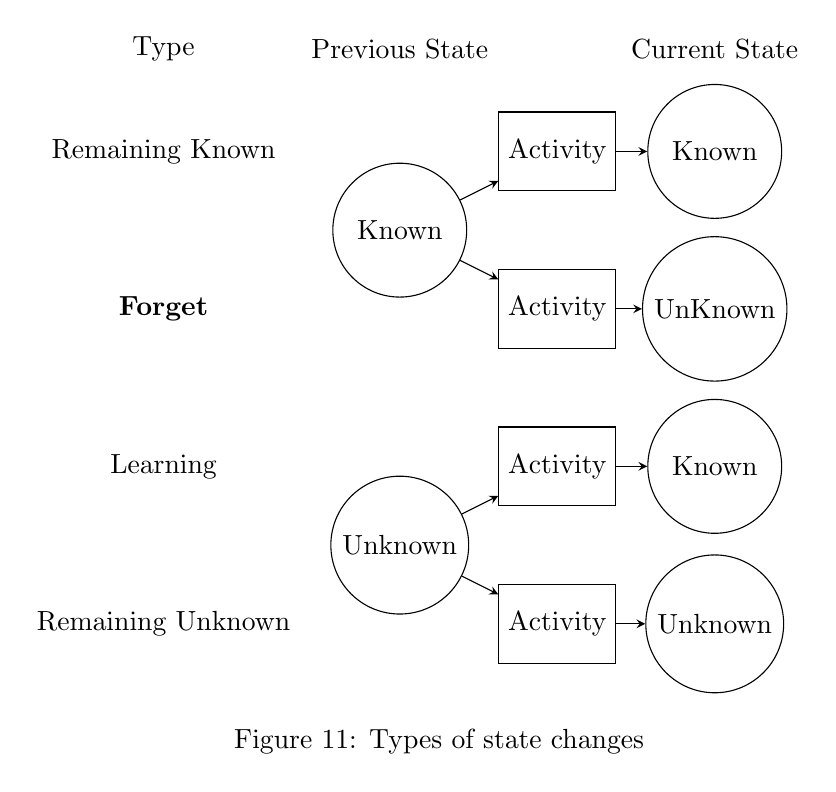
\begin{tikzpicture}
        % Define styles
        \tikzset{
            state/.style={circle, draw, minimum size=1.7cm},
            activity/.style={rectangle, draw, minimum size=1cm},
            arrow/.style={->,>=stealth}
        }
        
        % Nodes
        \node[] () at (-3,3.3) {Type};
        \node[] () at (0,3.3) {Previous State};
        \node[] () at (4,3.3) {Current State};

        \node[] () at (-3,2) {Remaining Known};
        \node[state] (state_node_1) at (0,1) {Known};
        \node[activity] (activity_node_1) at (2,2) {Activity};
        \node[state] (state_node_2) at (4,2) {Known};

        \node[] () at (-3,0) {\textbf{Forget}};
        \node[activity] (activity_node_0) at (2,0) {Activity};
        \node[state] (state_node_0) at (4,0) {UnKnown};
        
        \node[] () at (-3,-2) {Learning};
        \node[state] (state_node_3) at (0,-3) {Unknown};
        \node[activity] (activity_node_2) at (2,-2) {Activity};
        \node[state] (state_node_4) at (4,-2) {Known};
        
        \node[] () at (-3,-4) {Remaining Unknown};
        % \node[state] (state_node_5) at (0,-4) {Unknown};
        \node[activity] (activity_node_3) at (2,-4) {Activity};
        \node[state] (state_node_6) at (4,-4) {Unknown};
        
        % Arrows
        \draw[arrow] (state_node_1) -- (activity_node_1);
        \draw[arrow] (state_node_1) -- (activity_node_0);
        \draw[arrow] (activity_node_1) -- (state_node_2);
        \draw[arrow] (activity_node_0) -- (state_node_0);
        \draw[arrow] (state_node_3) -- (activity_node_2);
        \draw[arrow] (activity_node_2) -- (state_node_4);
        \draw[arrow] (state_node_3) -- (activity_node_3);
        \draw[arrow] (activity_node_3) -- (state_node_6);
    
        % Footnote
        \node at (0.5,-5.5) {Figure 11: Types of state changes};
    \end{tikzpicture}
\end{center}

In LFB terminology, we add the following defines:

1. \textbf{Forget}  
The forget rate, \( P_f \), represents the probability that a learner transitions to the unknown state through forgetting.

LFB Updates \(\theta_{i+1}\) by incorporating the potential learning effect based on \(\theta'\) in a different way with BKT, considering the effect of forget change.

$$
\theta_{i+1} = \theta' \boldsymbol{P_f} + (1 - \theta') P_l    
$$

The mainflow of LFB is illustrated in Figure 12. Note there are forget parameters $P_f$ in use.

\begin{center}
    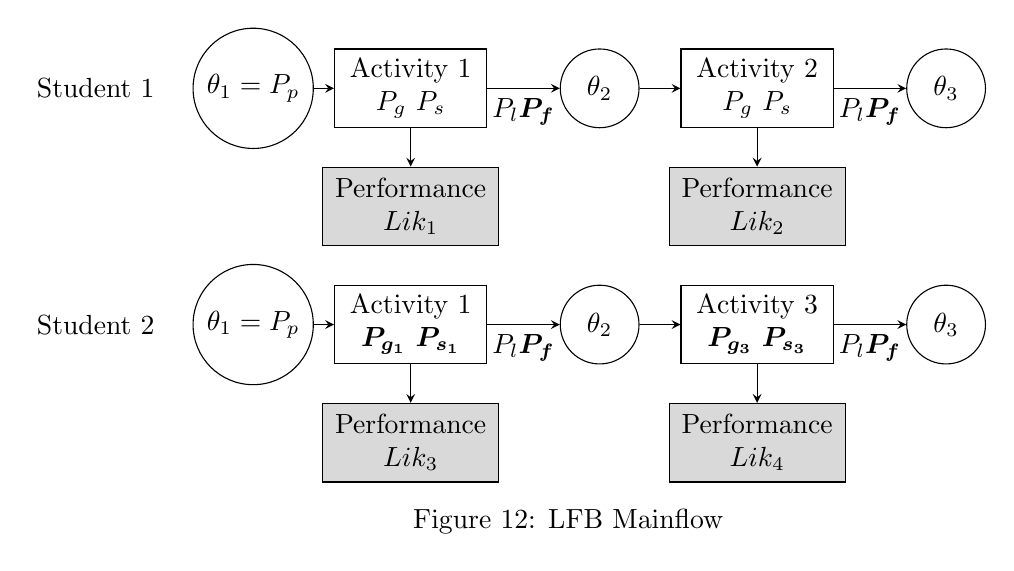
\begin{tikzpicture}
        % Define styles
        \tikzset{
            state/.style={circle, draw, minimum size=1cm},
            activity/.style={rectangle, draw, minimum size=1cm},
            performance/.style={rectangle, draw, fill=gray!30, minimum size=1cm},
            arrow/.style={->,>=stealth}
        }
        
        % Nodes
        \node[] () at (-2,0) {Student 1};
        \node[state] (state_node_1) at (0,0) {$\theta_1 = P_p$};
        \node[activity] (activity_node_1) at (2,0) {\parbox{1.7cm}{\centering Activity 1 \\ ${P_{g} \ P_{s}}$}};
        \node[performance] (performance_node_1) at (2,-1.5) {\parbox{2cm}{\centering Performance \\ $Lik_1$}};
        \node[state] (state_node_2) at (4.4,0) {$\theta_2$};
        
        \node[activity] (activity_node_2) at (6.4,0) {\parbox{1.7cm}{\centering Activity 2 \\ ${P_{g} \ P_{s}}$}};
        \node[performance] (performance_node_2) at (6.4,-1.5) {\parbox{2cm}{\centering Performance \\ $Lik_2$}};
        \node[state] (state_node_3) at (8.8,0) {$\theta_3$};
        
        % Arrows
        \draw[arrow] (state_node_1) -- (activity_node_1);
        \draw[arrow] (activity_node_1) -- (state_node_2) node[midway, below] {$P_l \boldsymbol{P_f}$};
        \draw[arrow] (activity_node_1) -- (performance_node_1);
        \draw[arrow] (state_node_2) -- (activity_node_2);
        \draw[arrow] (activity_node_2) -- (state_node_3) node[midway, below] {$P_l \boldsymbol{P_f}$};
        \draw[arrow] (activity_node_2) -- (performance_node_2);
    

        % student 2
        \node[] () at (-2,-3) {Student 2};
        \node[state] (state_node_2) at (0,-3) {$\theta_1 = P_p$};
        \node[activity] (activity_node_2) at (2,-3) {\parbox{1.7cm}{\centering Activity 1 \\ $\boldsymbol{P_{g_1} \ P_{s_1}}$}};
        \node[performance] (performance_node_2) at (2,-4.5) {\parbox{2cm}{\centering Performance \\ $Lik_3$}};
        \node[state] (state_node_3) at (4.4,-3) {$\theta_2$};
        \node[activity] (activity_node_3) at (6.4,-3) {\parbox{1.7cm}{\centering Activity 3 \\ $\boldsymbol{P_{g_3} \ P_{s_3}}$}};
        \node[performance] (performance_node_3) at (6.4,-4.5) {\parbox{2cm}{\centering Performance \\ $Lik_4$}};
        \node[state] (state_node_4) at (8.8,-3) {$\theta_3$};
        \draw[arrow] (state_node_2) -- (activity_node_2);
        \draw[arrow] (activity_node_2) -- (state_node_3) node[midway, below] {$P_l \boldsymbol{P_f}$};
        \draw[arrow] (activity_node_2) -- (performance_node_2);
        \draw[arrow] (state_node_3) -- (activity_node_3);
        \draw[arrow] (activity_node_3) -- (state_node_4) node[midway, below] {$P_l \boldsymbol{P_f}$};
        \draw[arrow] (activity_node_3) -- (performance_node_3);

        % Footnote
        \node at (4,-5.5) {Figure 12: LFB Mainflow};
    \end{tikzpicture}
\end{center}
\section{Estimation}

To estimate the global parameters of the BKT model (\(P_p, P_l, P_s, P_g\)) that maximize the likelihood \(Lik\), we employ the expectation-maximization (EM) algorithm. This algorithm is particularly well-suited for the BKT model as it addresses the latent nature of the learner's knowledge state (\(\theta_i\)), which cannot be directly observed but significantly influences the observed responses.

The EM algorithm consists of two iterative steps: the Expectation (E-step) and the Maximization (M-step). These steps are repeated until convergence.

\subsection{E-step}
In the E-step, we calculate the expected values of the latent knowledge state (\(\theta_i\)) and the associated contributions to the likelihood based on the current estimates of the global parameters. Specifically, for each learner:

1. \textbf{Initialization}:
Set the initial knowledge state \(\theta_1 = P_p\).

2. \textbf{Forward Computation}:
For each activity \(i\) in the sequence, iteratively compute the known rate \(\theta_{i+1}\):

- First, update the known rate \(\theta'\) based on the observed answer \(a_i\) using Bayes' rule:
\[
\theta' = 
\begin{cases} 
    \frac{\theta_i P_s}{\theta_i P_s + (1 - \theta_i)(1 - P_g)}, & \text{if } a_i = 0 \\
    \frac{\theta_i (1 - P_s)}{\theta_i (1 - P_s) + (1 - \theta_i)P_g}, & \text{if } a_i = 1
\end{cases}
\]

- Then incorporate the learning effect to compute \(\theta_{i+1}\):
\[
\theta_{i+1} = \theta' + (1 - \theta')P_l
\]

3. \textbf{Likelihood Contribution}:
Compute the likelihood for each observed answer \(a_i\):
\[
Lik_i = 
\begin{cases} 
    P_s \theta_i + (1 - P_g)(1 - \theta_i), & \text{if } a_i = 0 \\
    (1 - P_s)\theta_i + P_g(1 - \theta_i), & \text{if } a_i = 1
\end{cases}
\]
Accumulate these likelihoods to update the total likelihood \(Lik\).

\subsection{M-step}
In the M-step, we maximize the expected likelihood with respect to the global parameters (\(P_p, P_l, P_s, P_g\)). This involves:

1. \textbf{Updating Prior (\(P_p\))}:

    The prior probability \(P_p\) is updated based on the expected initial knowledge state \(\theta_1\):
    \[
    P_p = \frac{1}{N} \sum_{j=1}^N \theta_1^{(j)},
    \]
    where \(N\) is the total number of learners, and \(\theta_1^{(j)}\) is the initial knowledge state of learner \(j\).

2. \textbf{Updating Learning Rate (\(P_l\))}:

    The learning rate \(P_l\) is updated based on the transitions from \(\theta'\) (updated state after observing \(a_i\)) to \(\theta_{i+1}\):
    \[
    P_l = \frac{\sum_{j=1}^N \sum_{i=1}^{T_j} \left( (1 - \theta_i^{(j)}) \cdot \theta_{i+1}^{(j)} \right)}{\sum_{j=1}^N \sum_{i=1}^{T_j} (1 - \theta_i^{(j)})},
    \]
    where \(T_j\) is the number of activities for learner \(j\).

3. \textbf{Updating Slip Rate (\(P_s\))}:

    The slip rate \(P_s\) is updated based on the proportion of incorrect answers when the learner is in the known state:
    \[
    P_s = \frac{\sum_{j=1}^N \sum_{i=1}^{T_j} \left( \theta_i^{(j)} \cdot (1 - a_i) \right)}{\sum_{j=1}^N \sum_{i=1}^{T_j} \theta_i^{(j)}},
    \]

4. \textbf{Updating Guess Rate (\(P_g\))}:

    The guess rate \(P_g\) is updated based on the proportion of correct answers when the learner is in the unknown state:
    \[
    P_g = \frac{\sum_{j=1}^N \sum_{i=1}^{T_j} \left( (1 - \theta_i^{(j)}) \cdot a_i \right)}{\sum_{j=1}^N \sum_{i=1}^{T_j} (1 - \theta_i^{(j)})},
    \]

\subsection{Iteration and Convergence}
The E-step and M-step are alternated until the likelihood \(Lik\) converges, i.e., when the change in \(\log Lik\) between iterations falls below a predefined threshold. At convergence, the global parameters (\(P_p, P_l, P_s, P_g\)) maximize the likelihood of the observed answer sequences under the BKT model.

By iteratively refining the parameter estimates and leveraging the hidden knowledge state dynamics, the EM algorithm ensures an efficient and robust estimation process for the BKT model.   

\section{Data Example}

The dataset comes from the Cognitive Tutor system (\cite{ritter2007cognitive}), an intelligent tutoring platform designed to improve students' mathematical abilities. 

The dataset includes detailed logs of 587 unique students' interactions with the Cognitive Tutor, which tracks the students' responses to a series of math problems associated with various knowledge components (KCs). In total, the dataset contains 16,857 observation records, capturing each student's attempts and their correctness for various problem items across the 12 KCs.

\subsection{Basic BKT Model Example with BKT R package}

\begin{lstlisting}[caption={R code to train a simple BKT model}]
library(BKT)

# Initialize the model with an optional seed
model <- bkt(seed = 42, num_fits = 1, parallel = FALSE)

# Fetch example data
fetch_dataset(model, "https://raw.githubusercontent.com/CAHLR/pyBKT-examples/master/data/ct.csv", ".")

# Train a simple BKT model on one skill in the CT dataset
result <- fit(model, data_path = "ct.csv", skills = "Plot non-terminating improper fraction")

# View the trained parameters
print(params(result))
\end{lstlisting}

The result will be shown as below: 

\begin{verbatim}
> print(params(result))
                                            skill   param   class    value
1        Plot non-terminating improper fraction  learns default 0.222808
2        Plot non-terminating improper fraction forgets default 0.000000
3        Plot non-terminating improper fraction guesses default 0.003382
4        Plot non-terminating improper fraction   slips default 0.322177
5        Plot non-terminating improper fraction   prior default 0.737443
\end{verbatim}

In the result, the first column is the name of the skills, the second column indicates the type of parameters, including \texttt{learns}, \texttt{forgets}, \texttt{guesses}, \texttt{slips}, and \texttt{prior}. The last column shows the estimated parameter value.

\subsection{IDE BKT Model Example with BKT R package}

Train a multiple guess and slip BKT model on multiple skills in the CT dataset. Switch parameter \texttt{multigs = TRUE} in the \texttt{fit} function.

Multiple Guess refers to the Item Difficulty Effect (IDE) Model.

\begin{lstlisting}[caption={R code to train a IDE BKT model}]
library(BKT)

# Initialize the model with an optional seed
model <- bkt(seed = 42, num_fits = 1, parallel = FALSE)

# Fetch example data
fetch_dataset(model, "https://raw.githubusercontent.com/CAHLR/pyBKT-examples/master/data/ct.csv", ".")

# Train a multiple guess BKT model on one skill in the CT dataset
result <- fit(model, data_path = "ct.csv", skills = c("Plot pi"), multigs = TRUE)

# View the trained parameters
print(params(result))
\end{lstlisting}

The result will be shown as below:

\begin{verbatim}
        skill   param   class    value
1  Plot pi  learns default 0.995657
2  Plot pi forgets default 0.000000
3  Plot pi guesses       1 0.000000
4  Plot pi guesses       2 0.000000
5  Plot pi guesses       3 0.000000
6  Plot pi guesses       4 0.000000
7  Plot pi guesses       5 0.000000
8  Plot pi guesses       6 0.000000
9  Plot pi guesses       7 0.000000
10 Plot pi guesses       8 0.000000
11 Plot pi guesses       9 0.000000
12 Plot pi guesses      10 0.000000
13 Plot pi   slips       1 0.577002
14 Plot pi   slips       2 0.220335
15 Plot pi   slips       3 0.246635
16 Plot pi   slips       4 0.426740
17 Plot pi   slips       5 0.238321
18 Plot pi   slips       6 0.560898
19 Plot pi   slips       7 0.381043
20 Plot pi   slips       8 0.477167
21 Plot pi   slips       9 0.235853
22 Plot pi   slips      10 0.472197
23 Plot pi   prior default 0.992952
\end{verbatim}

Note that the \texttt{class} column refers to different items.

\subsection{ILE BKT Model Example with BKT R package}

Train a multiple learn BKT model on multiple skills in the CT dataset. Switch parameter \texttt{multilearn = TRUE} in the \texttt{fit} function.

Multiple Learn refers to the Item Learning Effect (ILE) Model.

\begin{lstlisting}[caption={R code to train an ILE BKT model}]
library(BKT)

# Initialize the model with an optional seed
model <- bkt(seed = 42, num_fits = 1, parallel = FALSE)

# Fetch example data
fetch_dataset(model, "https://raw.githubusercontent.com/CAHLR/pyBKT-examples/master/data/ct.csv", ".")

# Train a multiple learn BKT model on one skill in the CT dataset
result <- fit(model, data_path = "ct.csv", skills = c("Plot pi"), multilearn = TRUE)

# View the trained parameters
print(params(result))
\end{lstlisting}

The result will be shown as below:

\begin{verbatim}
     skill   param   class    value
1  Plot pi  learns       1 0.968846
2  Plot pi  learns       2 1.000000
3  Plot pi  learns       3 1.000000
4  Plot pi  learns       4 1.000000
5  Plot pi  learns       5 1.000000
6  Plot pi  learns       6 0.334115
7  Plot pi  learns       7 0.775121
8  Plot pi  learns       8 0.742444
9  Plot pi  learns       9 0.000000
10 Plot pi  learns      10 0.000372
11 Plot pi forgets       1 0.000000
12 Plot pi forgets       2 0.000000
13 Plot pi forgets       3 0.000000
14 Plot pi forgets       4 0.000000
15 Plot pi forgets       5 0.000000
16 Plot pi forgets       6 0.000000
17 Plot pi forgets       7 0.000000
18 Plot pi forgets       8 0.000000
19 Plot pi forgets       9 0.000000
20 Plot pi forgets      10 0.000000
21 Plot pi guesses default 0.000000
22 Plot pi   slips default 0.352701
23 Plot pi   prior default 0.936924
\end{verbatim}

Note that the \texttt{class} column refers to different items.


\subsection{LFB BKT Model Example with BKT R package}

Train a forget BKT model on the CT dataset. Switch parameter \texttt{forgets = TRUE} in the \texttt{fit} function. 

Forget refers to the Learning and Forgetting Behavior (LFB) Model.

\begin{lstlisting}[caption={R code to train a LFB BKT model}]
library(BKT)

# Initialize the model with an optional seed
model <- bkt(seed = 42, num_fits = 1, parallel = FALSE)

# Fetch example data
fetch_dataset(model, "https://raw.githubusercontent.com/CAHLR/pyBKT-examples/master/data/ct.csv", ".")

# Train a forget BKT model on one skill in the CT dataset
model = Model(seed = 42, num_fits = 1, parallel = FALSE)
model.fit(data_path = 'ct.csv', forgets = TRUE, skills = 'Plot terminating proper fraction')

# View the trained parameters
print(model.params())
\end{lstlisting}

The result will be shown as below:

\begin{verbatim}
                             skill   param   class    value
1 Plot terminating proper fraction  learns default 0.087497
2 Plot terminating proper fraction forgets default 0.054892
3 Plot terminating proper fraction guesses default 0.285785
4 Plot terminating proper fraction   slips default 0.329848
5 Plot terminating proper fraction   prior default 0.622707
\end{verbatim}

\section{Discussion}
\section{Conlusion}

% Reference
\printbibliography

\end{document}
